\documentclass{beamer}[10]
\usepackage{pgf}
\usepackage[english]{babel}
\usepackage[utf8]{inputenc}
\usepackage{beamerthemesplit}
\usepackage{graphics,epsfig, subfigure}
\usepackage{url}
\usepackage{srcltx}
\usepackage{hyperref}
\usepackage{enumitem}
\usepackage[round]{natbib}

\definecolor{kugreen}{RGB}{50,93,61}
\definecolor{kugreenlys}{RGB}{132,158,139}
\definecolor{kugreenlyslys}{RGB}{173,190,177}
\definecolor{kugreenlyslyslys}{RGB}{214,223,216}
\setbeamercovered{transparent}
\mode<presentation>
\usetheme[numbers,totalnumber,compress,sidebarshades]{PaloAlto}
\setbeamertemplate{footline}[frame number]
\usecolortheme[named=kugreen]{structure}
\useinnertheme{circles}
\usefonttheme[onlymath]{serif}
\setbeamercovered{transparent}
\setbeamertemplate{blocks}[rounded][shadow=true]

\logo{\includegraphics[width=0.8cm]{figures/umatlogo}}
%\useoutertheme{infolines} 
\title[]{DEVELOPMENT OF AN EFFICIENT PUBLIC TRANSPORT SEARCH PORTAL FOR GHANA}
\author[]{ENOCK SETH NYAMADOR \newline \small{SUPERVISED BY DR HAMIDU ABDEL-FATAO}}
\institute[]{COMPUTER SCIENCE AND ENGINEERING DEPARTMENT \\ UNIVERSITY OF MINES AND TECHNOLOGY}
\date{\today}



\begin{document}
	\frame{\titlepage \vspace{-0.5cm}
	}
	
	\frame
	{
		\frametitle{OVERVIEW}
		\tableofcontents%[pausesection]
	}
	
	\section{Problem Definition}
	
	\frame{
		\frametitle{PROBLEM DEFINITION}
			\begin{itemize}[label=$ \bullet $]
				\item Road transport is the major means of transportation in Ghana \citep{aidoo_passengers_2013}
				\vspace{0.3cm}
				\item Over $ 95\% $ of all passenger and freight traffic and about $ 97\% $ of all passenger miles in Ghana is by road \citep{unesco_transportation:_????}
				\vspace{0.3cm}
				%\item Vast majority of passengers commuting between places mostly rely on public transport services in the form of privately owned or corporate taxis, \textit{tro tros} (shared minivans), buses commuting between major cities \citep{abane2011travel}
				\item Privately owned or corporate taxis, \textit{tro tros} (shared minivans), buses commuting between major cities \citep{abane2011travel}
				\vspace{0.3cm}
				\item Difficulty in finding terminals specific location and detailed information
				\vspace{0.3cm}
				\item Fares and stations keep changing
			\end{itemize}
	}


	\frame{
		\frametitle{PROBLEM DEFINITION (CONT'D)}
		\begin{block}{Figure 1: Kaneshie Transport Terminal}
					\begin{figure}
					\centering
					\includegraphics[width=1\linewidth]{figures/kaneshe}
%					\caption{}
					\label{fig2:kaneshe}
					\end{figure}
		\end{block}
	}
		
		\frame{
		\frametitle{STATE OF PUBLIC TRANSPORT IN GHANA - PROBLEM DEFINITION (CONT'D)}
		\begin{itemize}[label=$ \star $]
			\item The transport industry is currently dominated by the 
			informal sector which provides about 90\% of transport services but their services are unreliable and uncomfortable \cite{bonaventura_assessment_2015}
			\vspace{0.5cm}
			\item Individually or privately operated transport services are members of unions or
			associations. These unions and associations serve as regulatory and mouth-piece
			to each of their members \citep{fouracre1994public}
		\end{itemize}
		
	}
	
	
	\section{Project Objectives}
	\frame{
		\frametitle{PROJECT OBJECTIVES}
%		\begin{block}{This project seeks to:}
			\begin{itemize}[label=$ \star $]
				\item To develop a web application that provides detailed information about public transport routes in Ghana
%				\begin{itemize}[label=$ \ast $]
%					\item To mitigate the difficulty in finding transport terminals and improve trip planning
%					\item To provide reusable data and a cross platform system by implementing a geospatial database containing exact location of transport terminals
%				\end{itemize}
			\end{itemize}
%		\end{block}
	}
	
	\section{Tools Used}

\frame{
	\frametitle{TOOLS USED}
%	\begin{block}{The tools used for this project are:}
		\begin{itemize}[label=$ \star $]
			\item Python
			\vspace{0.5cm}
			\item Django
			\vspace{0.5cm}
			\item Material Kit
			\vspace{0.5cm}
			\item PostgreSQL
			\vspace{0.5cm}
			\item QGIS
			\vspace{0.5cm}
			\item Leaflet and OpenStreetMap
			\vspace{0.5cm}
			\item GPS receiver and Smartphone
		\end{itemize}
%	\end{block}
}

	
	\section{Methodology}
	
	\frame{
		\frametitle{METHODOLOGY}
%		\begin{block}{Methods used for this project:}
			\begin{itemize}[label=$ \ast $]
				\item Review of related literature
				\vspace{0.5cm}
				\item Conducting feasibility studies
				\vspace{0.5cm}
				\item Requirements gathering and Analysis
				\vspace{0.5cm}
				\item Functional and non-functional requirements
				\vspace{0.5cm}
				\item Data Collection
		\end{itemize}
%	\end{block}
	}
		
%	\section{Results and discussion}
%	\frame{
%		\frametitle{RESULTS AND DISCUSSION}
%		\begin{itemize}[label=$ \star $]
%			\item User registers as a student selecting his hall of residence and institution.
%			\item User can purchase any listed product or book any service
%			\item User is able to join the live chat room on the home page of the application
%			\item A user can create his/her own shop and post products,billboards,Events and Personal skill.
%		\end{itemize}
%	}
	
%	\section{Analysis of Existing Systems}
%	
%	\frame{
%		\frametitle{ANALYSIS OF EXISTING SYSTEMS}
%		\begin{block}{	Although there exist systems with similar functionalities as this project, most of these existing systems:}
%		\begin{itemize}[label=$ \ast $]
%			\item Do not suit and focus on the Ghanaian transport system
%			\vspace{0.3cm}
%			\item Lack fare information
%			\vspace{0.3cm}
%			\item Are less reliable; E.g. Word of mouth
%			\vspace{0.3cm}
%			\item Are not frequently updated
%		\end{itemize}
%		\end{block}
%	}

\frame{
	\frametitle{REVIEW OF RELATED LITERATURE}
	\Large
	\begin{itemize}[label=$ \bullet $]
		\item \cite{neumann_toward_2015} have developed the first  minibus supply model based on demand and street network only in South Africa; leading to Taximap: a public transport search web portal
	\end{itemize}
}

	\frame{
	\frametitle{CONDUCTING FEASIBILITY STUDIES}
	\Large
\begin{block}{Areas Considered:}
	\begin{itemize}[label=$ \bullet $]
		\item Technical feasibility.
		\vspace{0.5cm}
		\item  Resource feasibility.
		\vspace{0.5cm}
		\item  Operational feasibility.
		\vspace{0.5cm}
		\item  Schedule feasibility.
	\end{itemize}
\end{block}
}
	
	\frame{
	\frametitle{REQUIREMENTS GATHERING AND ANALYSIS}
	\Large
	\begin{block}{Answers to these questions must be provided to ensure that the system can thrive:}
		\begin{itemize}[label=$ \star $]		
			\uncover<2->{\item Where is the system going to be used?}
			\uncover<3->{\item Who is going to use the system?}
			\uncover<4->{\item What data should be input into the system?}
			\uncover<5->{\item What Software Development Life Cycle(SDLC) model to be used?}
			\uncover<5->{\item What type of output information will the system give?}
		\end{itemize}
	\end{block}
	
}
	
		\frame{
		\frametitle{DATA COLLECTION}
		\Large
		\begin{itemize}[label=$ \ast $]
			\item Field survey 
			\item OpenStreetMap
			\item Crowd sourcing 
		\end{itemize}
		}
		
	\frame{
		\frametitle{FUNCTIONAL AND NON-FUNCTIONAL REQUIREMENTS}
		\begin{block}{Figure 2: Class Diagram}
		\begin{figure}
			\centering
			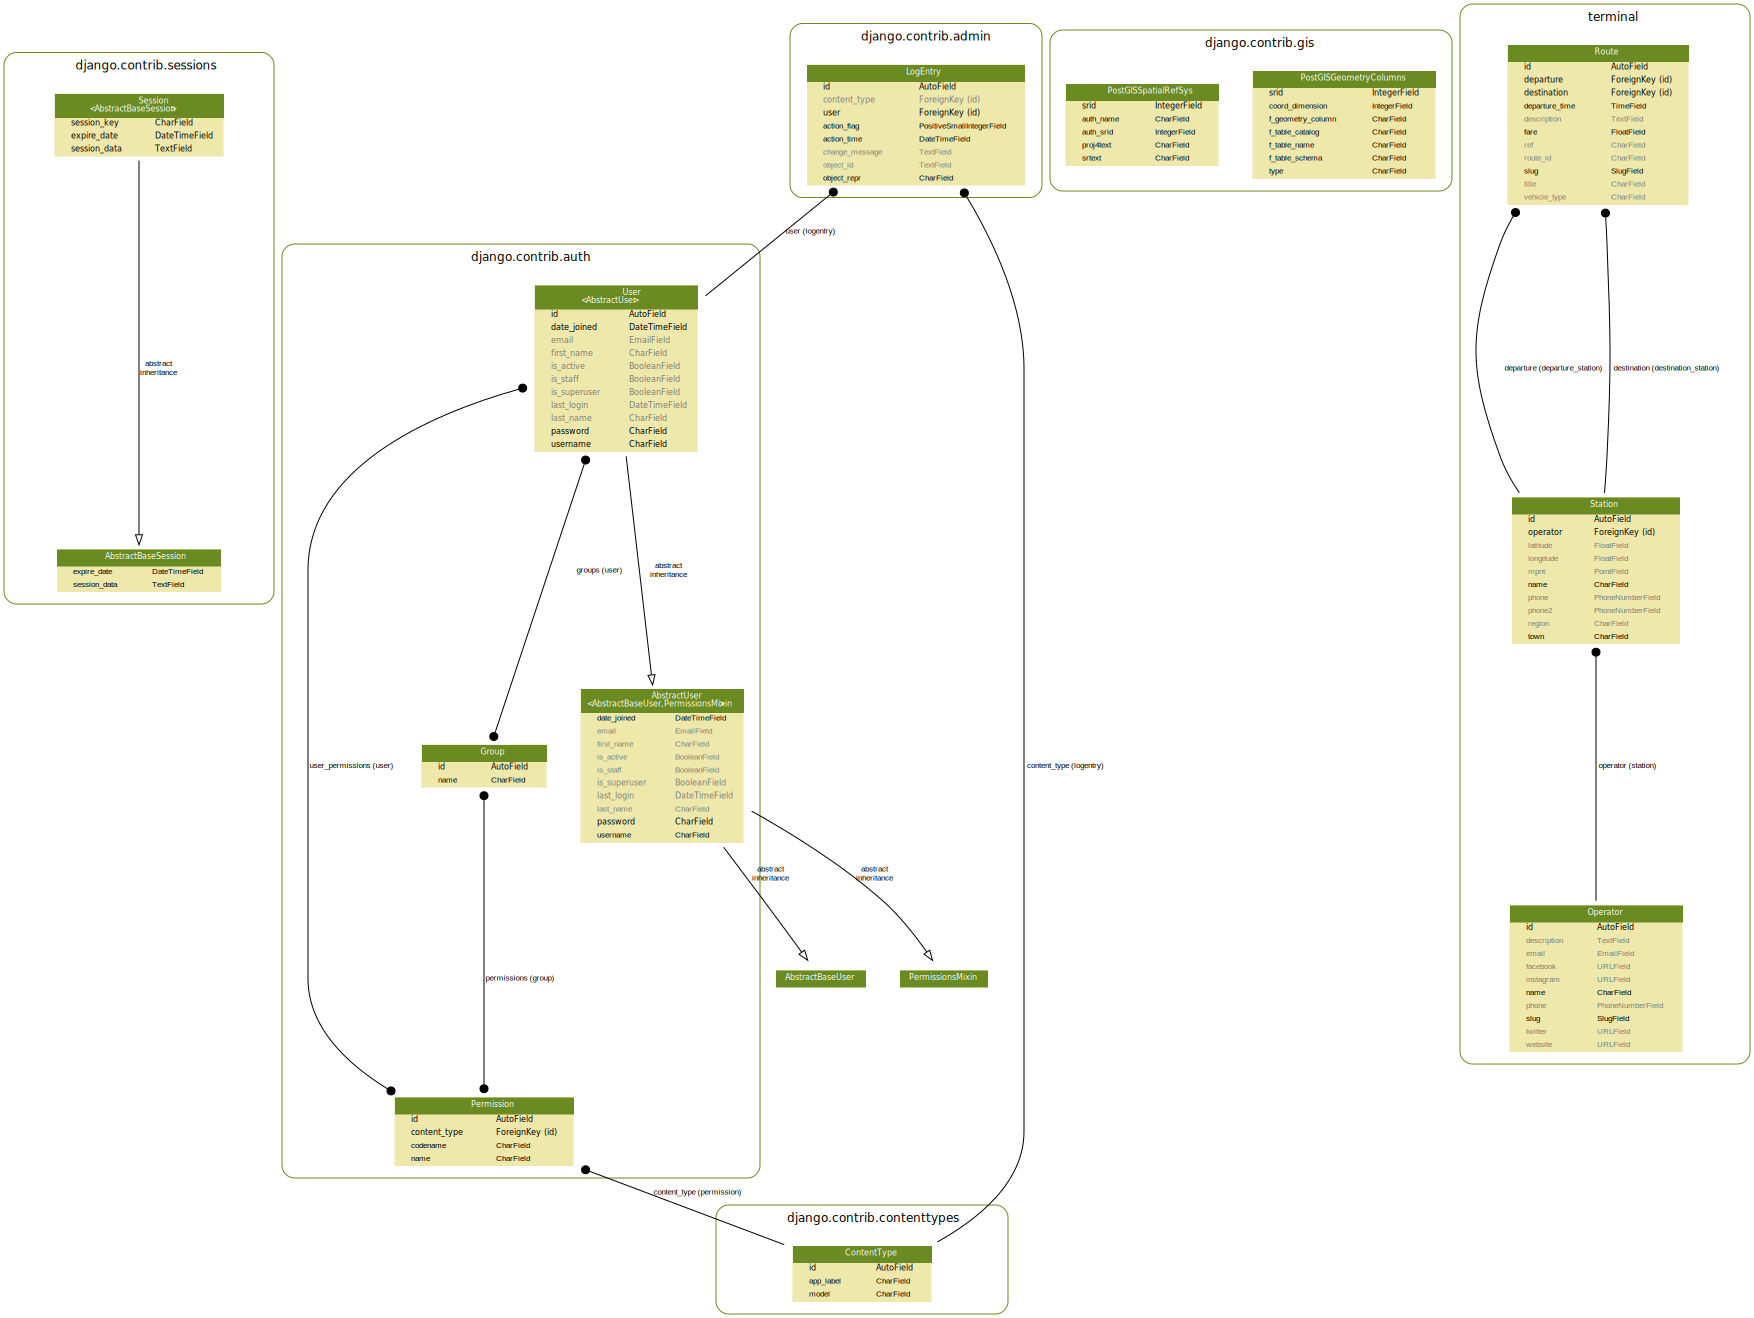
\includegraphics[width=1\linewidth]{figures/classdiagram}
			\label{fig:classdiagram}
		\end{figure}
	\end{block}
		
	}

	\frame{
	\frametitle{FUNCTIONAL AND NON-FUNCTIONAL REQUIREMENTS}
	\begin{block}{Figure 3: Use Case Diagram}
		\begin{figure}
			\centering
			\includegraphics[width=1\linewidth]{figures/usecase}
			\label{fig:usecase}
		\end{figure}
	\end{block}
	
}

	\frame{
	\frametitle{FUNCTIONAL AND NON-FUNCTIONAL REQUIREMENTS}
	\begin{block}{Figure 4: Activity Diagram}
		\begin{figure}
			\centering
			\includegraphics[width=0.5\linewidth]{figures/activitydiagram}
			\label{fig:activitydiagram}
		\end{figure}
	\end{block}
	
}

%\section{Behavioural Modeling Use Case Diagram}
%\frame{
%	\frametitle{BEHAVIOURAL MODELING USE CASE DIAGRAM}
%
%
%}
%

	\section{Results and Discussions}

\frame{
	\frametitle{RESULTS AND DISCUSSIONS}
	\begin{block}{The results and discussions:}
		\begin{itemize}[label=$ \star $]
			\item User gets routes based on destination and departure searched
			\item A user can access all available operators and view detailed information on each station
			\item User can compare fares visually
			\item A user is able to access station location in external platform
			\item Groups for managing staff privileges
			\item Detailed history of changes available in administration dashboard
		\end{itemize}	
	\end{block}
}

\section{Demonstration}

\frame{
	\frametitle{DEMONSTRATION}
	\centering
	{\Huge GHTP}
}

	\section{Conclusions and Recommendations}

\frame{
	\frametitle{CONCLUSIONS AND RECOMMENDATIONS}
	\begin{block}{It can be concluded that this system:}
		\begin{itemize}[label=$ \star $]
			\item Will improve trip planning and easy access to information only available within terminals to traveler hence saving time 
			\item Should be adopted by Ghana Tourism Authority to help tourists find their way around Ghana transport network
		\end{itemize}	
	\end{block}
\uncover<2->{
	\begin{block}{I would recommend that:}
	\begin{itemize}[label=$ \star $]
		\item Users should be able to book seats from the platform and also support voice input for the visually impaired
		\item The system could get users current location and find nearest possible departure stations for their routes
	\end{itemize}	
}
\end{block}

}


\frame{

		\small
		\frametitle{REFERENCES}
		\bibliographystyle{agsm}
		\bibliography{references}		

}


\frame{
	\frametitle{}
		\centering
		{\Huge THANK YOU}
}
	
\end{document}
